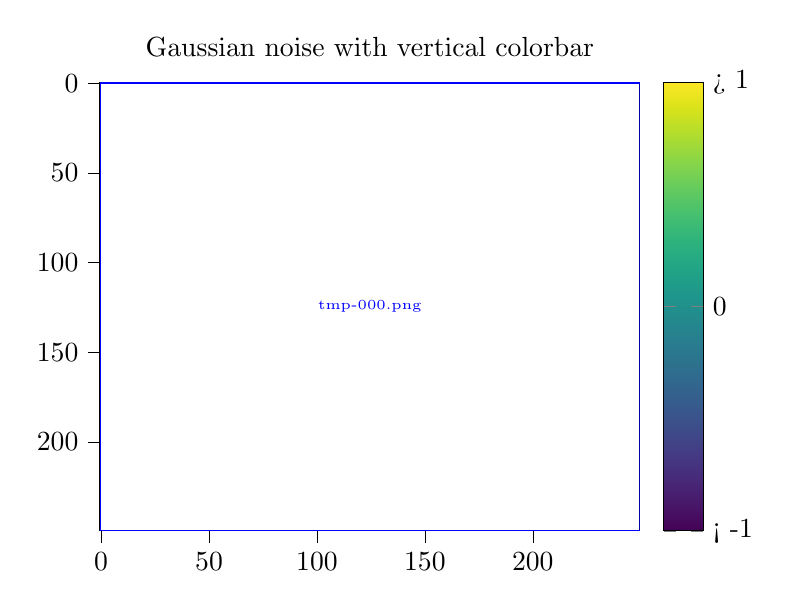
\begin{tikzpicture}

\begin{axis}[
colorbar,
colorbar style={ytick={-1,0,1},yticklabels={< -1,0,> 1},ylabel={}},
colormap/viridis,
point meta max=1,
point meta min=-1,
tick align=outside,
tick pos=left,
title={Gaussian noise with vertical colorbar},
x grid style={white!69.019608!black},
xmin=-0.5, xmax=249.5,
xtick style={color=black},
y dir=reverse,
y grid style={white!69.019608!black},
ymin=-0.5, ymax=249.5,
ytick style={color=black}
]
\addplot graphics [includegraphics cmd=\pgfimage,xmin=-0.5, xmax=249.5, ymin=249.5, ymax=-0.5] {tmp-000.png};
\end{axis}

\end{tikzpicture}
